\chapter{光的波动性}\label{chapter-wave-nature-of-light}

从古代起,人们就已经熟悉光现象了.但是,光究竟是什么
呢?这却是一个不容易回答的问题.人类对光的本性的认识,
经历了漫长而曲折的道路,有一个辩证发展的过程.
根据事
实建立学说,发展学说,或者决定学说的取舍;发现新的事实,
再建立新的学说.人们就是这样通过光的行为,经过分析研
究,逐渐认识光的本性的.

在这一章和下一章里,我们就基本上按照这种认识发展
过程来介绍关于光的本性的知识.

\section{光的微粒说和波动说}
光的本性问题很早就引起了人们的注意.到了十七世纪,
形成了两种学说.一种是牛顿主张的\NoteBold{微粒说},认为光是从光
源发出的一种物质微粒,在均匀媒质中以一定的速度传播.另
一种是惠更斯($1629 \sim 1695$)提出的\NoteBold{波动说},认为光是某种振
动,以波的形式向周围传播.

微粒说很容易解释光的直进现象,解释光的反射也很容
易,因为小球跟光滑平面发生弹性碰撞时的反射规律跟光的
反射定律相同.然而微粒说在解释一束光射到两种媒质分界
面处会同时发生反射和折射的现象时,却发生了很大的困难.
因为根据微粒说,光在镜面上发生反射,是由于光粒子受到镜
面的推斥;发生折射,是由于受到折射物质表面的吸引.在同
时发生反射和折射的情况下,又怎样用推斥和吸引来解释呢?
波动说却比较容易解释这种现象,因为人们知道这是波经常
发生的现象.用水槽和一些简单仪器做实验就可以看到水波
同时发生反射和折射的现象,并且可以查明水波的反射和折
射规律跟光非常相似.
然而波动说在解释光的直进现象时却
遇到了困难,因为人们知道波能够绕过障碍物,不会像光那样
在物体的后面留下清晰的影子.

光的微粒说和波动说当时各有成功的一面,但都不能完
满地解释当时知道的各种光现象.只是由于牛顿在学术界有
很高的声望,致使微粒说在一百多年的长时期里一直占着主
导地位,波动说发展得很慢.到了十九世纪初,人们成功地在
实验中观察到了光的干涉、衍射现象,这是波的特征,无法用
微粒说来解释,于是波动说得到了公认,光的波动理论也就迅
速发展起来.

下面我们就来研究表明光的波动性的各种现象.

\section{光的干涉}
我们在力学中学过了波的干涉,研究过水波和声波的干
涉现象.
我们知道,干涉是波特有的现象,只有频率相同、相
差恒定的波源——相干波源才能产生稳定的干涉现象.对于
水波或声波,相干波源是容易得到的.
但是,要找到符合相干
条件的两个相干光源却很困难.在室内点两支蜡烛或两盏电
灯,只看到墙壁被均匀照亮,丝毫看不到光的干涉现象.
当然,我们不应该因此就得出光不具有波动性的结论.
因为这
些光源都是独立发光的,甚至同一光源的两个发光部分,我们
也无法使它们具有相同的频率和恒定的相差,所以,即使光具
有波动性,这样的两个光源也不会产生稳定的干涉现象,无法
看到干涉图样.

\subsection{光的干涉}

1801年英国物理学家托马斯$\cdot$杨($1773 \sim 1829$)首先巧妙而简单地解决了相干光源的问题,成功地观察到
了光的干涉现象.


杨氏的办法是把点光源发出的一束光分成两束,以保证
它们具有相同的频率和恒定的相差.
实验做法如下.
让太阳
光照射到一个有小孔的屏上(图~\ref{fig_C_6-1}),这个小孔就成了一个
“点光源”.
光从小孔出来后,照射到第二个屏的两个小孔上,
这两个小孔离得很近,而且与前一小孔的距离相等.
因此,如
果光是某种波动,那么任何时刻从前一小孔发出的光波都会
同时传到这两个小孔,所以这两个小孔处的光振动不但频率
相同,而且总是同相的.这两个小孔就成了两个相干光源,它
们发出的光在像屏某处叠加时,如果同相,光就加强,如果反
相,光就减弱或抵消,因此应该产生明暗条纹.实验果然产生
了预期的结果,在像屏上看到了彩色的干涉条纹.
\begin{figure}[htbp]
	\centering
	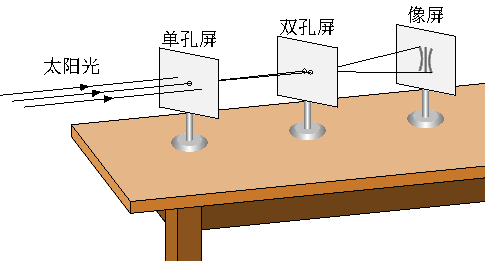
\includegraphics{fig/C/6-1.pdf}
	\caption{杨氏实验}\label{fig_C_6-1}
\end{figure}



后来用狭缝代替小孔,用单色光代替太阳光来做实验,得
到更清晰的明暗条纹,这就是著名的杨氏双缝干涉实验.图~\ref{fig_C_6-2} 
是双缝干涉的装置和产生干涉图样的示意图.
\begin{figure}[htbp]
    \centering
    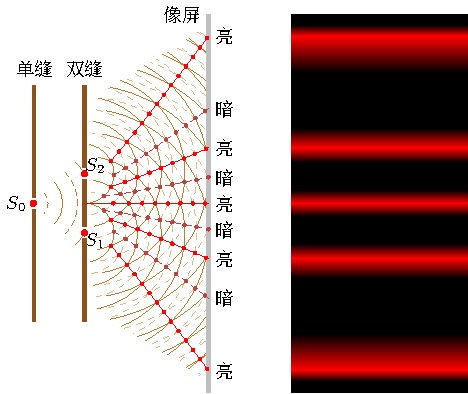
\includegraphics{fig/C/6-2.pdf}
    \caption{双缝干涉}\label{fig_C_6-2}
\end{figure}



微粒说不能解释光的干涉现象,波动说则可以作出完善
的解释,并能够根据双缝的距离和缝到屏的距离以及波长计
算出屏上出现明暗条纹的位置.图~\ref{fig_C_6-3} 是用波动说研究双缝
干涉的图.
设两个缝$S_1$和$S_2$的距离为$d$,到屏的距离为$\ell$,且
$\ell\gg d$.$O$是$S_1S_2$的中垂线与屏的交点,$O$到$S_1$、$S_2$的距离相
等.从$S_1$、$S_2$射出的光波到达$O$点经过的路程相等,所以两
列波到达$O$点时相差为零,也就是说,是同相的,它们互相加
强,在$O$点出现亮条纹,叫做中央亮纹.
现在我们来研究离$O$
点距离为$x$的$P$点的情况.$P$到$S_1$、$S_2$的距离分别为$r_1$、$r_2$.
从$S_1$、$S_2$发出的光波到达$P$点的路程差是
\[\delta =r_2-r_1 \]
从图中可以看出,
\[r^2_1=\ell^2+\qty(x-\frac{d}{2})^2,\qquad r^2_2=\ell^2+\qty(x+\frac{d}{2})^2  \]
两式相减,可得
\[r^2_2-r^2_1=(r_2-r_1)(r_2+r_1)=2dx\]
由于$\ell\gg d$,且$\ell\gg x$,因此$r_2+r_1\approx 2\ell$,所以
\[\delta=\frac{d}{\ell}x \]
如果路程差$\delta$等于波长$\lambda$的整数倍,两列波到达$P$点时同相,
因而互相加强,这里就出现亮条纹;如果路程差$\delta$等于半波长
$\lambda/2$的奇数倍,两列波到达$P$点时反相,因而互相削弱,这里
就出现暗条纹.
\begin{figure}[htbp]
	\centering
	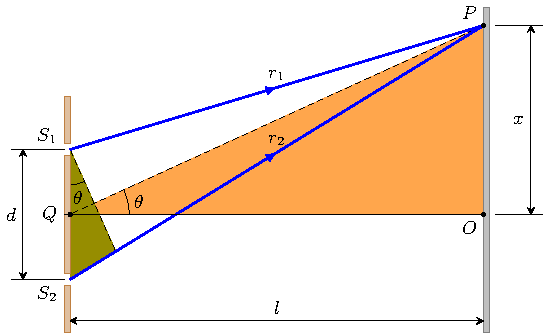
\includegraphics{fig/C/6-3.pdf}
	\caption{}\label{fig_C_6-3}
\end{figure}



所以,在屏上满足
\[x=\pm k\frac{\ell}{d}\lambda, \qquad k=0,1,2,\cdots \]
的地方出现亮条纹.当$k=0$时,$x=0$,为中央亮纹;当$k=1 $,$ 
2 $,$ \cdots$时,分别为中央亮纹两边的第1条、第2条$\cdots$亮条纹.

在满足
\[x=\pm(2k-1)\frac{\ell}{d}\cdot \frac{\lambda}{2},\qquad k=1,2,\cdots \]
的地方出现暗条纹.
当$k=1 $,$ 2 $,$ \cdots$时,分别为中央亮纹两边
的第1条、第2条$\cdots$暗条纹.

相邻两条亮纹(或暗纹)间的距离$\Delta x$为
\[\Delta x=\frac{\ell}{d}\lambda \]
可见,相邻两条亮纹(或暗纹)间的距离是相等的,从上式看
出,在$d$和$\lambda$相同的情况下,干涉条纹间的距离$\Delta x$跟波长$\lambda$
有关系.用不同的色光做实验,可以看到$\Delta x$的宽度不同,红
光的最宽,紫光的最窄(图~\ref{fig_C_0-3}).这表明不同色光的波长不
同,红光的波长最长,紫光的波长最短.用白光作光源时,由
于各色光的波长不同,$\Delta x$的宽度也不同,因此在中央白色亮
纹两边出现彩色条纹(图~\ref{fig_C_0-2}).

\begin{figure}[htbp]
	\centering
	\begin{minipage}[b]{0.53\linewidth}
		\centering
		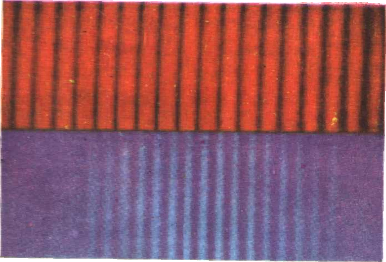
\includegraphics[height=3.2cm]{fig/C/0-3.pdf}
		\caption{红光和紫光通过双缝产生的干涉条纹}\label{fig_C_0-3}
	\end{minipage}
	\hfill
	\begin{minipage}[b]{0.45\linewidth}
		\centering
		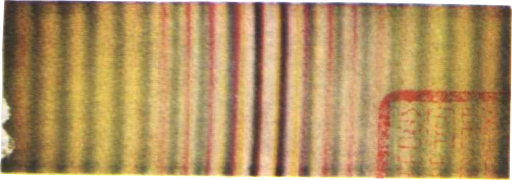
\includegraphics[height=2cm]{fig/C/0-2.png}
		\caption{白光通过双缝产生的干涉条纹}\label{fig_C_0-2}
	\end{minipage}
\end{figure}


上面的公式提供了一种测量光波波长的方法:测出$n$条
亮纹(或暗纹)间的距离$a$,算出相邻两条亮纹(或暗纹)间的
距离
\[\Delta x=\frac{a}{n-1} \]
再测出$d$和$\ell$的值,就可以算出波长$\lambda$.

\subsection{波长和频率}

我们知道,波长与频率的乘积等于波速.各
种色光在真空中的速度都等于$c$,如果用$\nu$表示光波的频率;
则有$c=\lambda\nu$.由于各种色光的波长不同,可见它们的频率也
不相同.红光的波长最长,频率最小;紫光的波长最短,频率
最大.表~\ref{tab_C_6-1} 是各种色光的频率和在真空中波长的范围.
\begin{table}[htbp]
	\centering
	\caption{}\label{tab_C_6-1}
    \begin{tblr}{colspec={ccc|ccc},cell{2-4}{2,3,5,6}={mode=math},cells={valign=m},}
        \toprule
        色光   &     {波长\\(微米)}    &    {频率\\($10^{14}$赫)}    &    色光    &    {波长\\(微米)}   &     {频率\\($10^{14}$赫)}     \\
        \midrule
        红   &  0.77 \sim 0.62   &     3.9 \sim 4.8    &    绿&0.58 \sim 0.49    &    5.2 \sim 6.1\\
        橙   & 0.62 \sim 0.60    &    4.8 \sim 5.0     &   蓝$\sim$靛    &    0.49 \sim 0.45    &    6.1 \sim 6.7\\
        黄&0.60 \sim 0.58   &     5.0 \sim 5.2     &   紫      &  0.45 \sim 0.39      &  6.7 \sim 7.7\\
        \bottomrule
    \end{tblr}
\end{table}

光的波长也常用埃($\UAiA$)作单位
\[1\UAi=10^{-10} \Um \]
但埃不是国际制单位.

\section{薄膜干涉及其应用}
\subsection{薄膜干涉}
把金属丝圆环在肥皂液里蘸一下,环上就形
成一层肥皂液薄膜.
用单色光照射薄膜,薄膜上就产生明暗相
间的干涉条纹(图~\ref{fig_C_6-4}).产生这种现象是由于照射到膜上的
光会从膜的前表面和后表面分别反射回来,形成两列波,这两
列波是由同一入射波产生的,因此频率相同,相差恒定,能够
产生干涉.
竖立的肥皂薄膜在重力作用下成为上薄下厚的楔
形,在薄膜的某些地方,反射回来的两列波恰好波峰和波峰
(或者波谷和波谷)叠加,光振动加强,产生亮条纹;在另外一
些地方,恰好波峰和波谷叠加,光振动削弱,产生暗条纹.
这就是薄膜干涉的原因.
\begin{figure}[htbp]
    \centering
    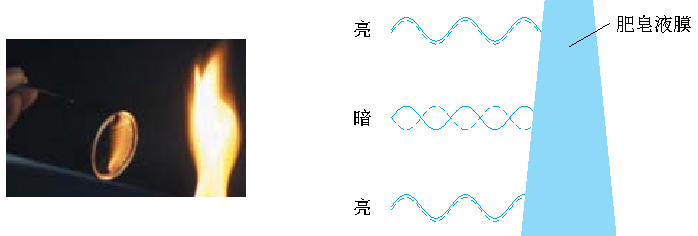
\includegraphics{fig/C/6-4.pdf}
    \caption{肥皂液膜上光的干涉}\label{fig_C_6-4}
\end{figure}


肥皂泡在太阳光照耀下会出现彩色的条纹,也是由薄膜
干涉产生的.白光中每种色光的波长不同,所以在薄膜某一厚
度的地方,某一波长的反射光互相加强,就出现这种色光的亮
纹;在另一厚度的地方,另一波长的反射光互相加强,就出现
另一色光的亮纹.
这样,在薄膜上就出现了不同颜色的条纹.

\subsection{检查精密零件的表面质量}


各种精密零件,例如光学元
件,对表面加工的质量要求很高,一般精度要求在几分之一光
波波长之内.
这样的表面需要用干涉法来检验.
如果被检查
的表面是一个平面,可以在它的上面放一个透明的标准样板,
并在一端垫一薄片,使样板的标准平面和被检查的平面间形
成一个劈形的空气薄层(图~\ref{fig_C_6-5a}).用单色光从上面照射,
入射光从空气层的上下表面反射出两列光波,于是从反射光
中就会看到干涉条纹.如果被测表面是平的,产生的干涉条
纹就是一组平行的直线;如果被测表面某些地方不平,产生的
干涉条纹就要发生弯曲(图~\ref{fig_C_6-5b}).从干涉条纹弯曲的方向
和程度还可以了解被测表面的不平情况.这种测量的精度可
达$10^{-6}$厘米.
\begin{figure}[htbp]
	\centering
	\begin{subfigure}{0.4\linewidth}
		\centering
		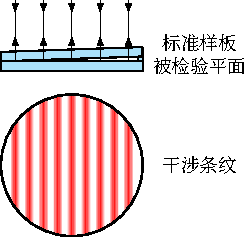
\includegraphics{fig/C/6-5a.pdf}
		\caption{}\label{fig_C_6-5a}
	\end{subfigure}
	\hfil
	\begin{subfigure}{0.4\linewidth}
		\centering
		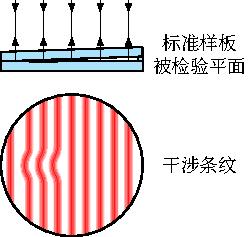
\includegraphics{fig/C/6-5b.pdf}
		\caption{}\label{fig_C_6-5b}
	\end{subfigure}
	\caption{用干涉法检查表面}\label{fig_C_6-5}
\end{figure}


\subsection{增透膜}

现代光学装置,如摄影机、电影放映机、潜水艇
的潜望镜等,都是由许多透镜和棱镜组成的.
光进入这些装
置时,在每个镜面上都有一部分光被反射,使得通过装置的光
减少,结果成的像就不清晰.
计算表明,如果一个装置中包含
有六个透镜,那么将有50\%左右的光被反射.
为了减少光在
元件表面上的反射损失,提高成像的质量,可在元件表面涂上
一层透明薄膜(一般用氟化镁).当薄膜厚度是入射光在薄膜
介质中波长的$1/4$
时,在薄膜的两个面上反射的光,路程差恰好
等于半个波长,因而互相抵消,这就大大减少了光的反射损
失,增强了透射光的强度.这种薄膜叫做增透膜.

在通常情况下入射光为白光,增透膜的厚度只能使一定
波长的光反射时互相抵消,不可能使白光中的所有波长的光
都互相抵消.在选择增透膜的厚度时,一般是使光谱中部的
绿光在垂直入射时互相抵消,因为人的视觉对这种光最敏感.
这时光谱边缘部分的红光和紫光并没有完全抵消,所以涂有
增透膜的光学镜头呈淡紫色.

\section*{阅读材料:全息照相}
同学们从报刊杂志上可能看到过全息照相这个名词,知
道全息照相是一种新的照相技术.
那么,什么是全息照相?它
与普通照相有什么不同?下面我们就来介绍一下这个问题.

我们知道,普通照相是把照相机的镜头对着被拍摄的物
体,让从物体上反射的光进入镜头,在感光底片上产生物体的
像.感光底片上记录的是从物体上各点反射出来的光的强
度.

但是,光是一种波,从被摄物体上各点反射出来的光不仅
强度(它正比于光波振幅的平方)不同,而且位相也不同.全
息照相就是一种既记录反射光的强度,又记录反射光的位相
的照相术.
这种照相术记录的是光波的振幅和位相的全部信
息,所以称为全息照相.


全息照相是应用光的干涉来实现的.它用激光(是良好
的相干光)作光源.
全息照相的原理如图~\ref{fig_C_6-6} 所示,激光束
被分成两部分:一部分射向被摄物体,另一部分射向反射镜
(这束光叫做参考光束).
从物体上反射出来的光(叫做物光
束)具有不同的振幅和位相,物光束和从反射镜来的参考光束
都射到感光片上,两束光发生干涉,在感光片上产生明暗的干
涉条纹,感光片就成了全息照片.干涉条纹的明暗记录了干
涉后光的强度,干涉条纹的形状记录了两束光的位相关系.
\begin{figure}[htbp]
	\centering
	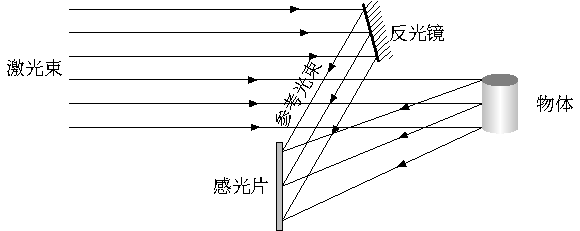
\includegraphics{fig/C/6-6.pdf}
	\caption{全息照相原理示意图}\label{fig_C_6-6}
\end{figure}


从全息照片的干涉条纹上不能直接看到物体的像,为了
现出物体的像,必须用激光束(参考光束)去照射全息照片,当
参考光束通过全息照片时,便复现出物光束的全部信息,于是
就能看到物体的像.

全息照相较之普通照相有许多优点.第一,它再现出来
的像是跟原来物体一模一样的逼真的立体像,跟观察实物完
全一样;第二,把全息照片分成若干小块,每一小块都可以完
整地现出原来物体的像,所以全息照片即使有缺损,也不会使
像失真;第三,在同一张感光片上可以重叠记录许多像,这些
像能够互不干扰地单独显示出来.

全息照相技术有重要的实际应用.
全息照相在一张感光
片上可以重叠记录许多像,这为信息的大容量高密度储存提
供了可能,例如用全息照相方法可以把一本几百页的书的内
容存储在只有指甲大小的全息照片上.全息照相在精密测量、
无损检验、显微术等方面也得到应用.
随着全息照相技术的
发展,它将会得到更广泛的应用.

\subsection*{练习一}

\begin{enumerate}
\item 绿光的干涉条纹与红光的干涉条纹有什么不同?用
白光做干涉实验,为什么会得到彩色的干涉条纹?在彩色条纹
中最靠近中央亮纹的是哪种颜色的条纹?为什么?
\item 在杨氏双缝实验中,保持双缝到屏的距离不变,调节
双缝间的距离,当距离增大时,干涉条纹间的距离将变\underline{\qquad};
当距离减小时,干涉条纹间的距离将变\underline{\qquad}.
\item 色光从真空进入媒质后,频率不变,但传播速度减小
了,波长将如何变化?
\item 用单色光做双缝干涉实验,测得双缝间的距离为0.4
毫米,双缝到屏的距离为1米,干涉条纹的间距为1.5毫米,
求所用光波的波长.
\item 取两块平玻璃板,用手指把它们紧紧捏在一起,会从
玻璃板面上看到许多彩色花纹;改变手指用力的大小,花纹的
颜色和形状也随着改变.
做这个实验,并解释看到的现象.
\end{enumerate}

\section{光的衍射}
\subsection{光的衍射}

我们知道,波能够绕过障碍物产生衍射,衍射
也是波特有的现象.并且知道只有障碍物或孔的尺寸跟波长
相差不多时,才能明显地观察到波的衍射现象.

光既然是一种波动,那么,光在传播中是否也能产生衍射
现象呢?从前面讲的光的干涉实验知道,光波的波长是很短
的,只有十分之几微米,通常的物体都比它大得多,因此很难
看到光的衍射现象.
但是,当光射向一个针孔、一条狭缝、一
根细丝时,就会出现衍射现象.

取一个不透光的屏,在屏中间开一个较大的圆孔.用点
光源照射,在像屏上就出现一个明亮的圆形光斑(图~\ref{fig_C_6-7a}).
显然,这是光沿直线传播的结果.圆孔小一些,可以看到像屏
上的光斑也随着减小(图~\ref{fig_C_6-7b}).但是,圆孔很小(直径小于
0.1毫米)时,像屏上的光斑不仅不减小,反而变大了,而且光
斑的亮度也变得不均匀,成为一些明暗相间的圆环(图~\ref{fig_C_6-7c}).
这些圆环的面积,远远超过了光按直线传播所能照到的
范围,就是说光绕到小孔以外的区域中去了.这就是光通过
小孔产生的衍射现象.
\begin{figure}[htbp]
    \centering
    \begin{subfigure}{0.8\linewidth}
        \centering
        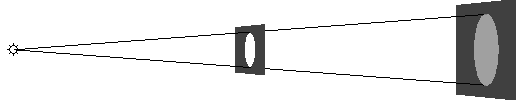
\includegraphics{fig/C/6-7a.pdf}
        \caption{}\label{fig_C_6-7a}
    \end{subfigure}
    \\
    \begin{subfigure}{0.8\linewidth}
        \centering
        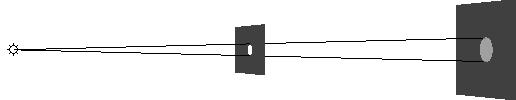
\includegraphics{fig/C/6-7b.pdf}
        \caption{}\label{fig_C_6-7b}
    \end{subfigure}
    \\
    \begin{subfigure}{0.8\linewidth}
        \centering
        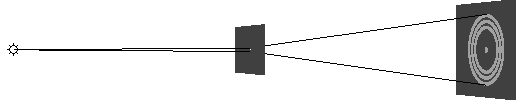
\includegraphics{fig/C/6-7c.pdf}
        \caption{}\label{fig_C_6-7c}
    \end{subfigure}
    \caption{光通过小圆孔的衍射}\label{fig_C_6-7}
\end{figure}

如果在不透明的屏上装一个宽度可以调节的狭缝,代替
上面实验中的小圆孔,重做实验,可以看到:当缝比较宽时,光
沿直线传播,在像屏上出现一条亮线;当缝很窄时,光通过缝
后就明显地偏离了直线传播的方向,像屏上被照亮的范围变
宽,并且出现了明暗相间的条纹.这是光通过狭缝时产生的
衍射现象.
图~\ref{fig_C_0-4} 和 \ref{fig_C_0-5} 是白光和红光通过同一狭缝产生的衍射条纹.
\begin{figure}[htbp]
	\centering
	\begin{minipage}[b]{0.48\linewidth}
		\centering
		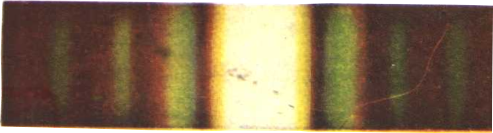
\includegraphics[height=1.6cm]{fig/C/0-4.png}
		\caption{白光通过单缝产生的衍射条纹}\label{fig_C_0-4}
	\end{minipage}
	\hfil
	\begin{minipage}[b]{0.48\linewidth}
		\centering
		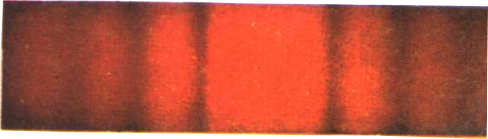
\includegraphics[height=1.6cm]{fig/C/0-5.png}
		\caption{红光通过单缝产生的衍射条纹}\label{fig_C_0-5}
	\end{minipage}
\end{figure}


光的衍射现象进一步证明了光具有波动性,对建立光的
波动说起了重要的作用.关于这个问题,历史上曾有过一段趣事.
十九世纪初,法国物理学家菲涅耳($1788 \sim 1827$)利用波
动理论对光的衍射现象作出了数学分析.
当时一位反对波动
说的数学家泊松($1781 \sim 1840$)从菲涅耳的分析得出结论:如果菲涅耳的理论是
正确的,那么把一个小的圆盘状物体放在光束中,在距这个圆
盘一定距离的像屏上,圆盘的影的中心应当出现一个亮斑.
人们从未看到过和听说过这种现象,因而认为这是荒谬的.于
是微粒说的拥护者们认为可以驳倒波动说了.菲涅耳接受了
这一挑战,精心研究,奇迹终于出现了,实验证明盘影的中心
确实有亮斑(图~\ref{fig_C_6-8}).微粒说无法解释这种奇特的现象,而
波动说却能作出完满的解释.菲涅耳的理论和实验使波动说
获得了巨大的成功.

\begin{figure}[htbp]
    \centering
    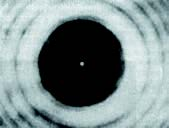
\includegraphics{fig/C/6-8.jpg}
    \caption{不透明盘产生的衍射,影子的中心有一个亮斑(泊松亮斑).}\label{fig_C_6-8}
\end{figure}

\subsection{衍射光栅}


光通过单狭缝产生的衍射条纹的位置跟光波
的波长有关,因此,利用衍射条纹也可以测定波长.但是单缝
的衍射条纹比较宽,测量的结果很不精确.为了精确测出光
波的波长,可以增加缝数.因为缝数增加以后,从各条单缝衍
射出来的光波要互相干涉,结果使明条纹变窄了.这个问题
的具体分析比较复杂,我们在这里就不讲了.从图~\ref{fig_C_6-9} 中可
以清楚地看到明条纹随着缝数增加而变窄的情形.
\begin{figure}[htbp]
	\centering
	\begin{subfigure}{0.4\linewidth}
		\centering
		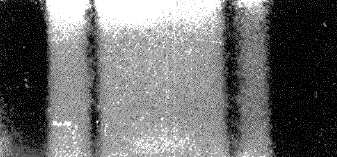
\includegraphics[width=3.5cm]{fig/C/6-9a.png}
		\caption{$1$缝}\label{fig_C_6-9a}
	\end{subfigure}
	\hfil
	\begin{subfigure}{0.4\linewidth}
		\centering
		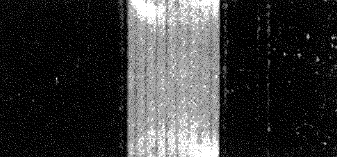
\includegraphics[width=3.5cm]{fig/C/6-9b.png}
		\caption{$2$缝}\label{fig_C_6-9b}
	\end{subfigure}
	\\
	\begin{subfigure}{0.4\linewidth}
		\centering
		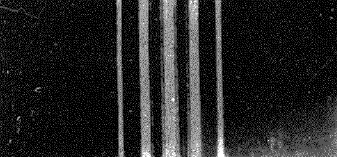
\includegraphics[width=3.5cm]{fig/C/6-9c.png}
		\caption{$5$缝}\label{fig_C_6-9c}
	\end{subfigure}
	\hfil
	\begin{subfigure}{0.4\linewidth}
		\centering
		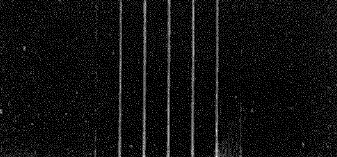
\includegraphics[width=3.5cm]{fig/C/6-9d.png}
		\caption{$20$缝}\label{fig_C_6-9d}
	\end{subfigure}
	\caption{衍射条纹随着缝数增加而变窄}\label{fig_C_6-9}
\end{figure}



光学仪器中用的衍射光栅就是根据这个原理制成的.常
用的透射光栅是在玻璃片上刻有许多等宽而又等间距的平行
刻痕,其中刻痕是不透光的部分(图~\ref{fig_C_6-10}).实用的衍射光栅
一般在每毫米内有几十条乃至上千条狭缝.光栅产生的衍射
条纹又窄又亮,可以精确地测
定光波的波长.
不同波长的光
通过光栅后产生的衍射条纹的
位置不同,因此,利用光栅可以
把不同波长的色光分开,就是
说,光栅跟棱镜一样具有分光
作用,用它可以产生光谱,这也
是光栅的一个用途.
\begin{figure}[htbp]
    \centering
    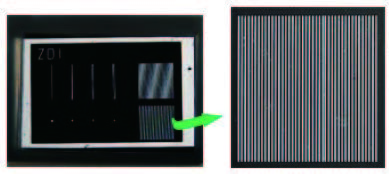
\includegraphics[height=3.8cm]{fig/C/6-10.jpg}
    \caption{衍射光栅}\label{fig_C_6-10}
\end{figure}

\subsection*{练习二}
\begin{enumerate}
\item 为什么隔着墙能听到墙那边人的说话声,但看不见
人?
\item 光的衍射现象跟光的直线传播是否矛盾?在什么情
况下光沿直线传播?
\item 把两支铅笔并在一起,中间留一条狭缝,放在眼前,
透过这条狭缝去看远处的日光灯,使狭缝的方向跟灯管平行,
就看到许多条平行的彩色条纹.
做这个实验,并解释看到的
现象.
\end{enumerate}

\section{光的偏振}

光的干涉和衍射现象清楚地表明光是一种波.
我们知道,
波有纵波和横波,这两种波都能够产生干涉和衍射现象,那
么,光波究竟是纵波还是横波呢?
\begin{figure}[htbp]
    \centering
    \begin{subfigure}{0.45\linewidth}
        \centering
        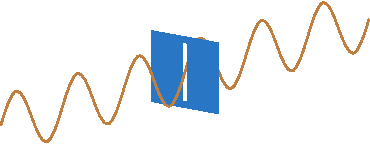
\includegraphics{fig/C/6-11a.pdf}
        \caption{}\label{fig_C_6-11a}
    \end{subfigure}
    \hfil
    \begin{subfigure}{0.45\linewidth}
        \centering
        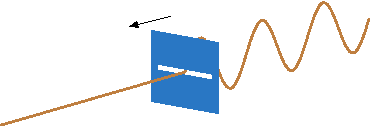
\includegraphics{fig/C/6-11b.pdf}
        \caption{}\label{fig_C_6-11b}
    \end{subfigure}
    \caption{横波的偏振}\label{fig_C_6-11}
\end{figure}

我们先用机械波来说明纵波和横波的主要区别.
沿着绳
传播的横波,如果在它传播的方向上放上带有狭缝的木板(图~\ref{fig_C_6-11}),
只要狭缝的方向跟绳的振动方向相同,绳上的横波就
可以毫无阻碍地传过去;如果把狭缝的方向旋转90$^\circ$,绳上的
横波就不能通过了.
这种现象叫做横波的\NoteBold{偏振}.纵波是沿着
波的传播方向振动的,不论狭缝方向如何,纵波都可以传过
去,不会发生偏振现象(图~\ref{fig_C_6-12}).
\begin{figure}[htbp]
    \centering
    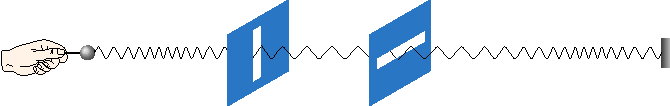
\includegraphics{fig/C/6-12.pdf}
    \caption{纵波没有偏振现象}\label{fig_C_6-12}
\end{figure}

光是否产生偏振现象呢?十九世纪法国科学家马吕(1$775 \sim 1812$)发现,光也能够产生偏振现象.
我们可以用下面的方
法来观察这一现象.

取一块电气石晶体薄片或人造偏振片\footnote{常用的一种人造偏振片是把聚乙烯醇薄膜在碘溶液里浸泡
后,在较高的温度下拉伸,再烘干制成的.},通过它观察太
阳光或灯光,可以看到它是透明的.以入射光线为轴旋转晶
片,这时看到的透射光的强度并不发生变化.
再取一个同样
的晶片,把它放在前一晶片的后面,通过它去观察从前一晶片
透射过来的光,就会发现,从第二个晶片透射过来的光的强度
跟两晶片的相对方向有关.
把前一晶片固定,以入射光线为
轴旋转后一晶片时,从后一晶片透射过来的光的强度发生周
期性的变化:后一晶片转到某一方向时,透射光最强(图~\ref{fig_C_6-13a});
再旋转90$^\circ$,转到跟前一方向垂直时,透射光最弱,几乎
等于零(图~\ref{fig_C_6-13b}).
\begin{figure}[htbp]
    \centering
    \begin{subfigure}{0.8\linewidth}
        \centering
        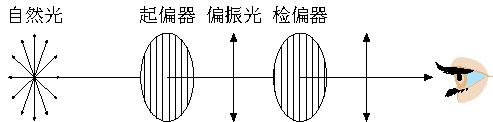
\includegraphics{fig/C/6-13a.pdf}
        \caption{}\label{fig_C_6-13a}
    \end{subfigure}
    \\
    \begin{subfigure}{0.8\linewidth}
        \centering
        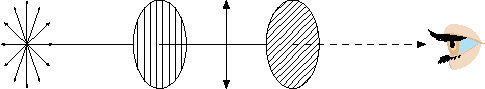
\includegraphics{fig/C/6-13b.pdf}
        \caption{}\label{fig_C_6-13b}
    \end{subfigure}
    \caption{光的偏振}\label{fig_C_6-13}
\end{figure}

把上述光现象跟机械波的偏振现象相比较,表明光通过
晶片时产生偏振现象.只有横波才产生偏振现象,所以光波
是横波.

上面实验中的现象可以解释如下.太阳、电灯等普通光
源发出的光,包含着在垂直于传播方向上沿一切方向振动的
光,并没有一个占优势的方向,也就是说,沿着各个方向振动
的光波强度都相同.
这种光叫做\NoteBold{自然光}.自然光通过第一个
晶片(叫做起偏器)后,相当于被一个“狭缝”卡了一下,只有振
动方向跟“狭缝”方向一致的光波才能通过(图~\ref{fig_C_6-13}),这种振
动方向一定的光叫做\NoteBold{偏振光}.每个偏振片上都有一条标线,表
示的就是偏振片允许通过的偏振光的振动方向,这个方向叫
做偏振片的偏振化方向.
自然光通过第一个晶片后虽然变成
了偏振光,但由于自然光中沿各个方向振动的光波强度都相
同,所以不论晶片转到什么方向,都会有相同强度的光透射过来.
再通过第二个晶片(叫做检偏器)去观察,情形就不同了.
不论旋转哪个晶片,两晶片的偏振化方向一致时,透射光最
强,两晶片的偏振化方向互相垂直时,透射光最弱.

光的偏振现象并不是罕见的.
我们通常看到的绝大部分
光,除了从光源直接射来的,基本上都是偏振光,只是我们眼
睛不能鉴别罢了.
如果通过偏振片去观察从玻璃或水面反射
的光,旋转偏振片,就会发现透射光的强度也发生周期性的变
化,从而知道反射光是偏振光.

光的偏振现象在技术中有很多应用.
例如,在拍摄水面
下的景物或展览橱窗中的陈列品的照片时,由于从水面或窗
玻璃会发出很强的反射光,使得水面下的景物和橱窗中的陈
列品看不清楚,摄出的照片也模糊不清.如果在照相机镜头
上加一个偏振片,使偏振片的偏振化方向与反射光的垂直,就
可以把这些反射光滤掉,而摄得清晰的照片.
汽车在夜间行
车时,迎面开来的车灯的光常常使司机看不清路面,容易发生事故.
如果在每辆汽车的车灯玻璃上和司机座席前面的窗玻
璃上各安上一块偏振片,并使它们的偏振化方向都跟水平方
向成45$^\circ$角(图~\ref{fig_C_6-14}),就可以解决这个问题.这时,从对面
车灯射来的偏振光,由于振动方向跟司机自己座前窗玻璃上
偏振片的偏振化方向垂直,所以不会射进司机眼里.而从自
已的车灯射出去的偏振光,由于振动方向跟自己的窗玻璃上
编振片的偏振化方向相同,所以司机仍能看清自己车灯照亮
的路面和物体.

\begin{figure}[htbp]
    \centering
    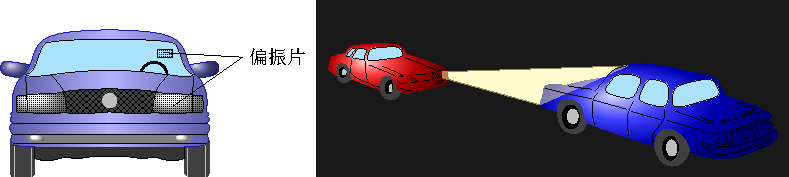
\includegraphics{fig/C/6-14.pdf}
    \caption{汽车车灯和窗玻璃上的偏振片}\label{fig_C_6-14}
\end{figure}

\section*{阅读材料:偏振光与立体电影}
看立体电影,要戴上一副特殊的眼镜,这样从银幕上看到
的人物和自然景物的影像才有立体感,犹如身临其境一般.如
果取下眼镜,银幕上的图像就模糊不清了.这是一副什么眼
镜?为什么能使我们看到的影像有立体感?学习了偏振光的知
识,就可以明白它的原理了.

为了说明立体电影的原理,首先得说说用两只眼睛看物
体跟用一只眼睛看物体的区别.
用两只眼睛看物体时,由于两
眼看到的同一物体略有差别,因而产生立体感.只用一只眼
睛看物体,就没有立体感.

普通电影是用一架摄影机拍摄,一架放映机放映的,银幕
上的画面是一幅平面图像.
立体电影是用两架摄影机并排在
一起,同时拍下同一景物的两幅图像,由于两架摄影机对景物
的角度不同,所以拍下的两幅图像略有差别,就如同两眼看到
的同一物体略有差别一样.
放映时,用两架放映机把两架摄
影机拍下的两组影片同步放映,使略有差别的两幅图像重叠
在银幕上.这时如果用眼睛直接观看,看到的画面是模糊不
清的,要看到立体电影,需要运用光的偏振知识,使两眼各看
到一幅图像.在每架放映机前装一块偏振镜(图~\ref{fig_C_6-15}),其作
用相当于起偏器,从两架放映机发出的带有影像的两束光,通
过偏振镜后,就成了偏振光.
左右两架放映机前的偏振镜的
偏振化方向互相垂直,因此产生的两束偏振光的偏振方向也
互相垂直.这两束偏振光投射到银幕上再反射到观众,偏振
方向不改变.观众戴的眼镜是一副偏光眼镜,相当于检偏器,
偏光眼镜的两只镜片的偏振化方向也是互相垂直的,而且左
眼镜片的偏振化方向跟左边放映机前偏振镜的一致,右眼镜
片的偏振化方向跟右边放映机前偏振镜的一致.这样,左眼
只能看到左机映出的画面,右眼只能看到右机映出的画面,两
眼看到的画面略有差别,因而产生立体感.
\begin{figure}[htbp]
    \centering
    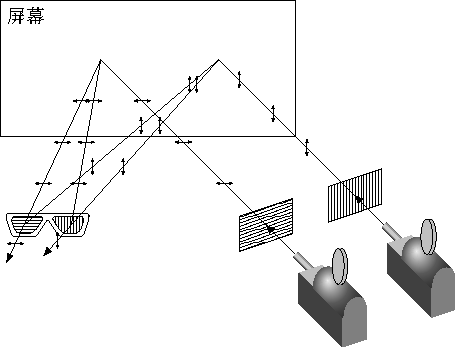
\includegraphics{fig/C/6-15.pdf}
    \caption{立体电影}\label{fig_C_6-15}
\end{figure}

\section{光的电磁说}
十九世纪初,杨氏、菲涅耳等对光的干涉和衍射的研究,
使光的波动说获得了很大的成功,逐渐为人们所接受.
物理学
家们继续发展和完善光的波动说,试图对光波作出进一步的
说明.当时人们只了解在媒质中传播的机械波,以为光波也
是这种机械波.但是,一切机械波,包括声波在内,都需要有
传播的媒质,在真空中是不能传播的.
光却能够在真空中传播,
从太阳和其他恒星发出的光,能够穿过辽阔的宇宙空间传到
地球上来.那么,光是通过什么媒质传过来的呢?为了说明光
的传播问题,人们曾假设在宇宙空间里到处都充满着一种特
殊的物质,叫做“以太”,认为光是通过“以太”传播的.为了解
释光波是横波、光波传播的速度很大、光波在不同媒质中的传
播速度不同等问题,对“以太”这种物质的性质作了种种假设,
例如,“以太”的密度应该非常小,但是又应该具有很大的弹性.
对“以太”性质所作的假设有些是互相矛盾的,很难使人
相信存在这样的物质.为了证明“以太”的存在,人们曾做过
各种实验,但是都失败了.
这使得认为光波是通过“以太”传
播的机械波的理论陷入了困境.

1846年,法拉第发现在磁场的作用下,偏振光的振动面
会发生改变.这个发现很重要,它表明光和电磁现象间存在
着联系,启示人们把光现象和电磁现象联系起来考虑.

十九世纪六十年代,麦克斯韦在研究电磁场理论时预见
了电磁波,并且指出电磁波是横波,电磁波的传播速度等于光
速.麦克斯韦根据电磁波跟光波的这些相似性指出,光波是
一种电磁波,这就是\NoteBold{光的电磁说}.

二十多年以后,赫兹用实验证实了电磁波的存在,测得电
磁波的传播速度确实等于光速,而且电磁波也能产生反射、折
射、干涉、衍射、偏振等现象,其规律都跟光波的相同.这就从
实验上证实了光是一种电磁波.

前面第四章已经讲过,电磁波跟机械波不同,电磁波可以
在真空中传播,不需要依靠别的媒质.这就解决了光波在传
播媒质上所遇到的困难.

麦克斯韦提出的光的电磁说,在物理学的发展中有很重
要的意义.
它把光现象和电磁现象统一起来,指出了它们的一
致性,再一次证明了自然现象之间是相互联系的.
光的电磁
说使人们对光的本性的认识前进了一大步.

\section{电磁波谱}
我们已经知道,无线电波是电磁波,其波长范围从几十千
米到几毫米.
现在又知道了光波也是电磁波,其波长不到1微
米.可见,电磁波是一个很大的家族,包括的波长范围很大.
光波里能够作用于我们的眼睛并引起视觉的部分,只是一个
很窄的波段,通常也叫做可见光.正像在可闻声波范围外还
存在着大量的听不见的超声波和次声波一样,在可见光波范
围外还存在着大量的看不见的红外线和紫外线.

\subsection{红外线}

红外线是英国物理学家赫谢耳在1800年发现
的,他用灵敏温度计研究光谱里各种色光的热作用时,把温度
计移到光谱的红光区域外侧,它的温度上升得更高,说明那里
有看不见的射线照射到温度计上.
这种射线后来就叫做\NoteBold{红外线}.
给电炉丝通电,电炉丝的温度大约上升到$500\Ucede$以上时,
才开始发出暗红色的光,随着温度的升高,它逐渐变成橙色、
黄色;但在电炉丝发光之前,我们就已感到热了.
这就是它发
射了红外线的缘故.一切物体都可以发射红外线,温度较高
的物体发出的红外线也较多.

红外线在工业、农业、军事、科研以及人民生活中都有广
泛的应用,红外线技术已发展成为一门现代科学技术.
红外线最显著的作用是热作用,所以可以利用红外线来加热,红外
线炉、红外线烤箱、红外线干燥器等,都是利用红外线来加热
的.这种加热方法的优点是能使物体从内部发热,加热效率
高,效果好.利用对红外线敏感的底片可以进行远距离摄影
和高空摄影.
从卫星上用红外线对地面摄影,从照片上可以
清晰地看出地面上的城市、街道、桥梁和房屋,这种摄影不受
白天和夜晚的限制.利用红外成像技术可以制成军事上用的
夜视仪,使人们在漆黑的夜间能够看见目标.
一切物体,包
括大地、云雾、冰块、人体、飞机和车船,都在不停地辐射红
外线,并且不同的物体辐射的红外线的波长和强度不同,利用
灵敏的红外线探测器吸收物体发出的红外线,然后用电子仪
器对接收到的信号进行处理,就可以察知被探测物体的特征.
这种技术叫做\NoteBold{红外线遥感}.利用红外线遥感技术,可以在飞
机或卫星上勘测地热、寻找水源、监测森林火情、估计农作物
的长势和收成、预报台风寒潮等.红外线遥感技术的应用范
围极其广泛,还在迅速发展中.

\subsection{紫外线}

紫外线是德物理学家里特在1801年发现的.
如果在光谱的紫外区域放一张照相底片,或者放一个光敏电
阻,都能够察知\NoteBold{紫外线}的存在.紫外线的波长比紫光还短.一
切高温物体,如太阳、弧光灯发出的光都含有紫外线,利用气
体放电也可以激发紫外线.紫外线的主要作用是化学作用.
紫外线很容易使照相底片感光.用紫外线照相能辨认出细微
差别,例如可以清晰地分辨出留在纸上的指纹.紫外线有很
强的荧光效应,能使许多物质激发荧光.
日光灯和农业上诱
杀害虫用的黑光灯,都是用紫外线来激发荧光物质发光的.
紫外线还有杀菌消毒作用.
医院里常用紫外线来消毒病房和手
术室.
紫外线还能促进生理作用和治疗皮肤病、软骨病等.
经常在矿井下劳动的工人,适当地照射紫外线,能促进身体健
康.但过强的紫外线能伤害人的眼睛和皮肤.
电焊的弧光中
有强烈的紫外线,因此电焊工在工作时必须穿好工作服,并戴
上防护面罩.

\subsection{伦琴射线}
比紫外线波长还短的电磁波,有\NoteBold{伦琴射线}.德
国物理学家伦琴($1845 \sim 1923$)在1895年研究阴极射线的性质
时,发现阴极射线的高速电子流射到玻璃管壁上,管壁会发出
一种看不见的射线,这种射线的穿透本领很大,能使放在厚纸
后面的荧光物质铂氰化钡发出荧光,并能使包在黑纸里的照
相底片感光.
伦琴当时不知道这是什么射线,把它叫做$\rm{X}$射
线.后来人们做了大量实验,发现高速电子流射到任何固体
上,都会产生这种射线,并且从它产生的衍射现象知道它是波
长很短的电磁波.为了纪念伦琴,就把这种射线叫做伦琴射线.
图~\ref{fig_C_6-16} 是产生伦琴射线的装置,叫做伦琴射线管.图中
的螺旋钨丝$K$是它的阴极,用钨或铂制成的电极$A$是它的阳
极,又叫对阴极.管里的真空程度很高,气压约为$10^{-3} \sim 10^{-5}$
帕($10^{-5} \sim 10^{-7}$毫米汞柱).
用电池组或变压器给钨丝$\rm{K}$通
电,钨丝达到赤热状态就向周围发射电子.
把管的阴阳两极
接到几万伏的高压电源上,管内就产生很强的电场.
炽热钨
丝发出的电子在电场力的作用下以很大的速度射到对阴极
上,就从那里激发出相当强的伦琴射线.伦琴射线穿透物质
的本领跟物质的密度有关系,在工业上可以用它来检查金属
部件有没有砂眼、裂纹等缺陷,在医学上可以用它来透视人
体,检查体内的病变和骨折的情况.
\begin{figure}[htbp]
    \centering
    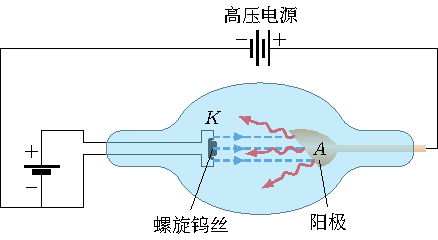
\includegraphics{fig/C/6-16.pdf}
    \caption{伦琴射线管}\label{fig_C_6-16}
\end{figure}

此外,还有比伦琴射线波长更短的电磁波,那就是放射性
元素放出的$\gamma$射线,我们将在第\ref{chapter-atomic-nucleus}章学习.

\subsection{电磁波谱}

无线电波、红外线、可见光、紫外线、伦琴射
线、$\gamma$射线合起来,构成了范围非常广阔的\NoteBold{电磁波谱}(图~\ref{fig_C_6-17}),其中最长的波长是最短的波长的$10^{21}$倍以上.
从图中
可以看出,各种电磁波的范围已经衔接起来,并且发生了交错.
例如长波的红外线和微波已经重叠,短波的紫外线已经
进入伦琴射线的区域.
总的说来,从无线电波到$\gamma$射线,都是
本质上相同的电磁波,它们的行为服从共同的规律.另一方
面,由于它们的频率或波长不同而又表现出不同的特性,例
如,波长较长的无线电波,很容易表现出干涉、衍射等现象,但
对波长越来越短的可见光、紫外线、伦琴射线、$\gamma$射线,要观察
到它们的干涉、衍射现象,就越来越困难了.

\begin{figure}[htbp]
    \centering
    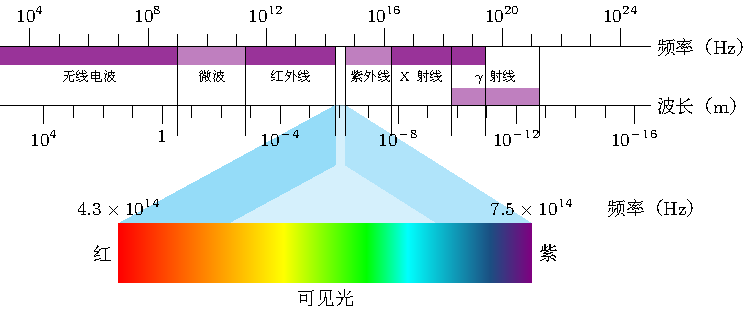
\includegraphics{fig/C/6-17.pdf}
    \caption{电磁波谱}\label{fig_C_6-17}
\end{figure}

不同的电磁波产生的机理不同.
无线电波是振荡电路中
自由电子的运动产生的;红外线、可见光、紫外线是原子的外
层电子受到激发后产生的;伦琴射线是原子的内层电子受到
激发后产生的;$\gamma$射线是原子核受到激发后产生的.

\section{光谱}
光波是由原子内部运动的电子产生的.
各种物质的原子
内部电子的运动情况不同,所以它们发射的光波也不同.研
究不同物质的发光和吸收光的情况,有重要的理论和实际意
义,已成为一门专门的学科——光谱学.
下面简单介绍一些
关于光谱的知识.

\subsection{分光镜}


观察光谱要用分光镜,这里我们先讲一下分光
镜的构造原理.
图~\ref{fig_C_6-18} 是分光镜的构造原理示意图.它是
由平行光管$A$、三棱镜$P$和望远镜筒$B$组成的.平行光管$A$的
前方有一个宽度可以调节的狭缝$S$,它位于透镜$L_1$的焦平
面\footnote{通过焦点垂直于透镜主光轴的平面,叫做透镜的焦平面.}处.从狭缝射入的光线经透镜$L_1$折射后,变成平行光线
射到三棱镜$P$上.不同颜色的光经过三棱镜沿不同的折射方
向射出,并在透镜$L_2$后方的焦平面$MN$上分别会聚成不同
颜色的像(谱线).通过望远镜筒$B$的目镜$L_3$,就看到了放大
的光谱像.如果在$MN$那里放上照相底片,就可以摄下光谱的像.
具有这种装置的光谱仪器叫做摄谱仪.
\begin{figure}[htbp]
	\centering
	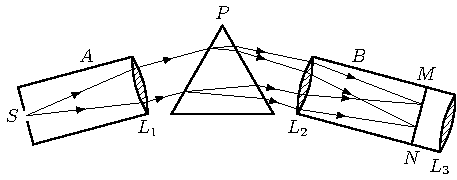
\includegraphics{fig/C/6-18.pdf}
	\caption{分光镜构造原理示意图}\label{fig_C_6-18}
\end{figure}



\subsection{发射光谱}

物体发光直接产生的光谱叫做\NoteBold{发射光谱}.发
射光谱有两种类型;连续光谱和明线光谱.

连续分布的包含有从红光到紫光各种色光的光谱叫做\NoteBold{连续光谱}(图~\ref{fig_C_0-6-7-8-9}).
炽热的固体、液体和高压气体的发射光谱
是连续光谱.例如电灯丝发出的光、炽热的钢水发出的光都
形成连续光谱.

\begin{figure}[htbp]
	\centering
	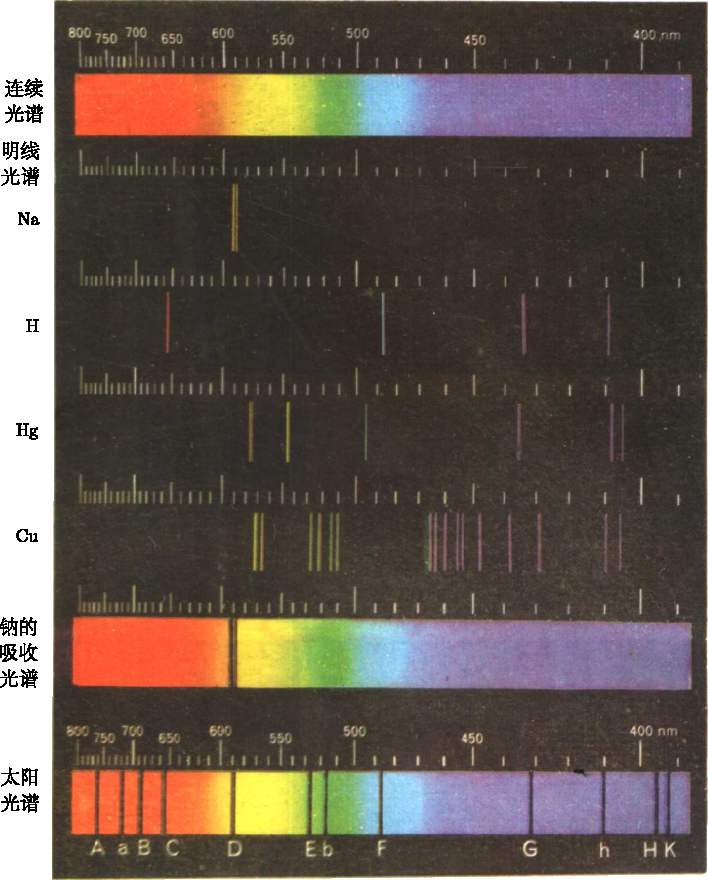
\includegraphics{fig/C/0-6-7-8-9.pdf}
	\caption{}\label{fig_C_0-6-7-8-9}
\end{figure}


只含有一些不连续的亮线的光谱叫做\NoteBold{明线光谱}(图~\ref{fig_C_0-6-7-8-9}).
明线光谱中的亮线叫做谱线,各条谱线对应于不同波长的光.
稀薄气体或金属的蒸气的发射光谱是明线光谱.明线光谱是
由游离状态的原子发射的,所以也叫\NoteBold{原子光谱}.


观察气体的原子光谱,可以使用光谱管(图~\ref{fig_C_6-19}),它是
一支中间比较细的封闭的玻璃管,里面装有低压气体,管的两
端有两个电极.把两个电极接到高压电源上,管里稀薄气体发
生辉光放电,产生一定颜色的光.
\begin{figure}[htbp]
	\centering
	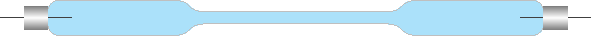
\includegraphics{fig/C/6-19.pdf}
	\caption{光谱管}\label{fig_C_6-19}
\end{figure}



观察固态或液态物质的原子光谱,可以把它们放到煤气
灯的火焰或电弧中去烧,使它们气化后发光,就可以从分光镜
中看到它们的明线光谱.

实验证明,原子不同,发射的明线光谱也不同,每种元素
的原子都有一定的明线光谱.
几种元素($\rm{Na}$、$\rm{H}$、$\rm{Hg}$、$\rm{Cu}$)的明线光谱见图~\ref{fig_C_0-6-7-8-9}.
每种原子只能发出具有本身特征的某些波长的光,因此,
明线光谱的谱线叫做原子的\NoteBold{特征谱线}.利用原子的特征谱线
可以鉴别物质和研究原子的结构.

\subsection{吸收光谱}
高温物体发出的白光(其中包含连续分布的
一切波长的光)通过物质时,某些波长的光被物质吸收后产生
的光谱,叫做\NoteBold{吸收光谱}.例如,让弧光灯发出的白光通过温度
较低的钠气(在酒精灯的灯心上放一些食盐,食盐受热分解就
会产生钠气),然后用分光镜来观察,就会看到在连续光谱的
背景中有两条挨得很近的暗线(见图~\ref{fig_C_0-6-7-8-9}.分光镜的分辨率本领不够高时,只能看见一条暗线).
这就是钠原子的吸收光谱.
值得注意的是,各种原子的吸收光谱中的每一条暗线都跟该种
原子的发射光谱中的一条明线相对应.
这表明,低温气体原
子吸收的光,恰好就是这种原子在高温时发出的光.因此,吸
收光谱中的谱线(暗线),也是原子的特征谱线,只是通常在吸
收光谱中看到的特征谱线比明线光谱中的少.

\subsection{光谱分析}

由于每种原子都有自己的特征谱线,因此可
以根据光谱来鉴别物质和确定它的化学组成.这种方法叫做\NoteBold{光谱分析}.
做光谱分析时,可以利用发射光谱,也可以利用吸
收光谱.这种方法的优点是非常灵敏而且迅速.某种元素在
物质中的含量达$10^{-10}$克,就可以从光谱中发现它的特征谱
线,因而能够把它检查出来.光谱分析在科学技术中有广泛
的应用.例如,在检查半导体材料硅和锗是不是达到了高纯
度的要求时,就要用到光谱分析.
在历史上,光谱分析还帮助
人们发现了许多新元素.
例如,铷和铯就是从光谱中看到了
以前所不知道的特征谱线而被发现的.光谱分析对于研究天
体的化学组成也很有用.十九世纪初,在研究太阳光谱时,发
现它的连续光谱中有许多暗线(参看图~\ref{fig_C_0-6-7-8-9},其中有一些主要暗线).
最初不知道这些暗线是怎样形成的,后来人们了解
了吸收光谱的成因,才知道这是太阳内部发出的强光经过温
度比较低的太阳大气层时产生的吸收光谱.仔细分析这些暗
线,把它跟各种原子的特征谱线对照,人们就知道了太阳大气
层中含有氢、氦、氮、碳、氧、铁、镁、硅、钙、钠等几十种元素.

\section*{复习题}
\begin{enumerate}
\item 十七世纪的光的波动说和微粒说各有什么成功之处
和不足之处?
\item 什么是光的干涉?什么是相干光源?
\item 薄膜干涉现象是怎样产生的?举例说明薄膜干涉现
象的应用.
\item 什么是光的衍射?日常生活中为什么不容易观察到
光的衍射现象?
\item 什么是光的偏振?光的偏振表明了什么?
\item 确立光的电磁说,根据是什么?
\item 无线电波、红外线、可见光、紫外线和伦琴射线,它们
的波长(或频率)有什么不同?
\item 发射光谱是怎样产生的?吸收光谱是怎样产生的?什
么叫特征谱线?光谱分析的原理是什么?
\end{enumerate}

\section*{习题}

\begin{enumerate}
    \item 你用哪些现象或实验来说明:
    \begin{enumerate}
        \item 光是一种波;
        \item 光波的波长非常短;
        \item 绿光的波长比红光的短.
    \end{enumerate}
    \item 水对真空中波长为0.656微米的红光的折射率为$n_1
    =1.33$,而对真空中波长为0.405微米的紫光的折射率为
    $n_2=1.343$.求这两种波在水中的传播速度和波长.
    \item 波长为5890埃的黄光照在一双缝上,在距双缝为1
    米的观察屏上,测得20个亮条纹的间距共宽2.4厘米,求双
    缝间的距离.
    \item 用波长为0.75微米的红光做双缝干涉实验,双缝间
    的距离是0.05毫米,缝到屏的距离是1米,相邻两条暗纹间
    的距离是多大?
\end{enumerate}



